\documentclass[a4paper,12pt]{article}
\usepackage[utf8]{inputenc}
\usepackage[spanish]{babel}
\usepackage{listings}
\usepackage{graphicx}
\usepackage{color}
\usepackage{amsmath}
\usepackage{hyperref}
\usepackage{array}
\usepackage{float}

\definecolor{codegreen}{rgb}{0,0.6,0}
\definecolor{codegray}{rgb}{0.5,0.5,0.5}
\definecolor{codepurple}{rgb}{0.58,0,0.82}
\definecolor{backcolour}{rgb}{0.95,0.95,0.92}

\lstdefinestyle{mystyle}{
    backgroundcolor=\color{backcolour},   
    commentstyle=\color{codegreen},
    keywordstyle=\color{magenta},
    numberstyle=\tiny\color{codegray},
    stringstyle=\color{codepurple},
    basicstyle=\ttfamily\footnotesize,
    breakatwhitespace=false,         
    breaklines=true,                 
    captionpos=b,                    
    keepspaces=true,                 
    numbers=left,                    
    numbersep=5pt,                  
    showspaces=false,                
    showstringspaces=false,
    showtabs=false,                  
    tabsize=2
}

\lstset{style=mystyle}

\title{Documentación Técnica Detallada:\\Sistema de Simulación y Optimización de Ruido en Edificios}
\author{Manual Técnico y de Usuario}
\date{\today}

\begin{document}

\maketitle
\tableofcontents

\newpage
\section{Introducción}
\subsection{Descripción General del Sistema}
Este sistema permite simular y optimizar la distribución de espacios en un edificio considerando la propagación del ruido. El programa:

\begin{itemize}
    \item Lee una configuración inicial desde un archivo JSON
    \item Simula la propagación física del ruido entre espacios
    \item Optimiza la distribución para minimizar problemas acústicos
    \item Genera visualizaciones 3D interactivas
    \item Produce reportes detallados con recomendaciones
\end{itemize}

\section{Estructura del Sistema}
\subsection{Carga Inicial del Edificio}
El sistema inicia cargando la configuración del edificio desde un archivo JSON que contiene:

\begin{itemize}
    \item \textbf{Datos de los espacios:}
    \begin{itemize}
        \item Nombre y tipo de espacio
        \item Posición (x,y,z) en el edificio
        \item Nivel de piso
        \item Características físicas (paredes, ventanas, puertas)
        \item Niveles de ruido base
        \item Frecuencias características
    \end{itemize}
    
    \item \textbf{Proceso de carga:}
    \begin{lstlisting}[language=Python]
    def inicializar_nodos(self):
        try:
            with open('edificio.json', 'r', encoding='utf-8') as f:
                data = json.load(f)
        except FileNotFoundError:
            QMessageBox.critical(self, "Error", 
                "El archivo 'edificio.json' no se encontr\'{o}.")
            sys.exit(1)
    \end{lstlisting}
\end{itemize}

\subsection{Modelo de Nodos}
Cada espacio se representa como un nodo con las siguientes características:

\begin{itemize}
    \item \textbf{Atributos Físicos:}
    \begin{itemize}
        \item \texttt{name}: Identificador único del espacio
        \item \texttt{tipo}: Categoría (aula, biblioteca, etc.)
        \item \texttt{position}: Coordenadas (x,y,z)
        \item \texttt{piso}: Nivel en el edificio
        \item \texttt{pared}: Presencia de paredes (booleano)
        \item \texttt{ventana}: Presencia de ventanas (booleano)
        \item \texttt{puerta}: Presencia de puertas (booleano)
    \end{itemize}

    \item \textbf{Atributos Acústicos:}
    \begin{itemize}
        \item \texttt{ruido}: Nivel base en decibelios (dB)
        \item \texttt{frecuencia}: Frecuencia característica (Hz)
        \item \texttt{es\_fuente}: Si es generador activo de ruido
    \end{itemize}

    \item \textbf{Conexiones:}
    \begin{itemize}
        \item Lista de nodos vecinos
        \item Conexiones bidireccionales automáticas
        \item Sensores de medición asociados
    \end{itemize}
\end{itemize}

\subsection{Modelado de Propagación del Ruido}
El cálculo del ruido total en cada espacio sigue un modelo físico que considera múltiples factores:

\begin{equation}
R_{total} = R_{base} + \sum_{i=1}^{n} (R_i \times A_i \times F_i \times E_i)
\end{equation}

Donde cada término representa:
\begin{itemize}
    \item $R_{base}$: Ruido propio del espacio (si es fuente)
    \item $R_i$: Ruido del vecino i
    \item $A_i$: Atenuación por distancia según ley cuadrática inversa
    \item $F_i$: Factor de atenuación por frecuencia
    \item $E_i$: Efectos estructurales combinados
\end{itemize}

\subsubsection{Atenuación por Distancia}
La atenuación sigue la ley cuadrática inversa:
\begin{equation}
A_d = \frac{1}{d^2}
\end{equation}
Donde $d$ es la distancia euclidiana entre espacios:
\begin{equation}
d = \sqrt{(x_2-x_1)^2 + (y_2-y_1)^2 + (z_2-z_1)^2}
\end{equation}

\subsubsection{Factor de Frecuencia}
La atenuación por frecuencia se calcula como:
\begin{equation}
F_f = min(1.0, \frac{1000}{f})
\end{equation}
Donde $f$ es la frecuencia en Hz. Este factor modela la mayor atenuación de altas frecuencias.

\section{Modelo de Clases}
\subsection{Diagrama de Clases}
\begin{figure}[H]
    \centering
    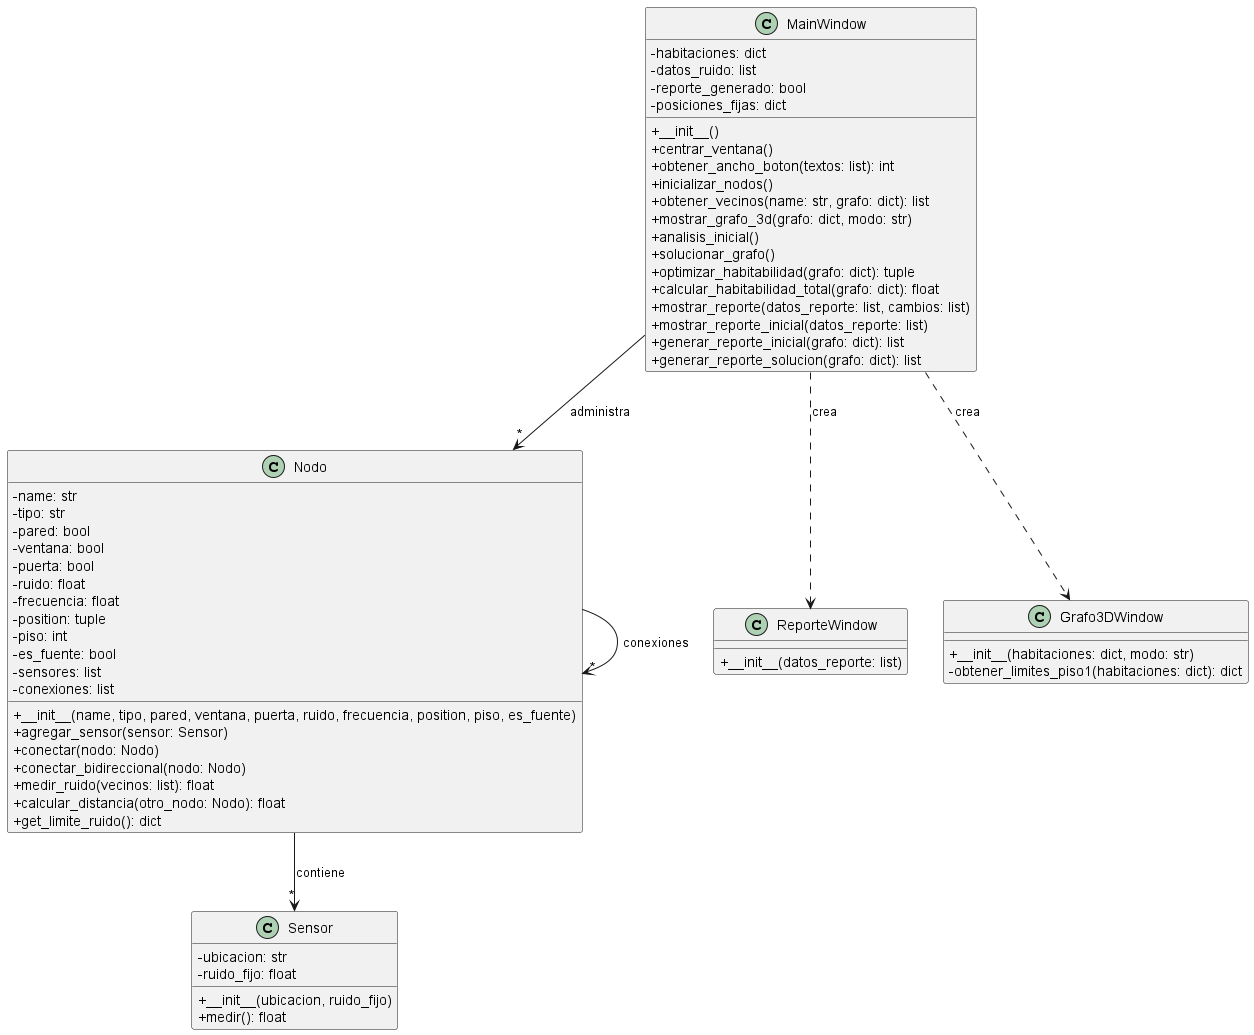
\includegraphics[width=\textwidth]{clases.png}
    \caption{Diagrama de Clases del Sistema}
    \label{fig:diagrama_clases}
\end{figure}

\subsection{Descripción de Clases}
\begin{itemize}
    \item \textbf{Nodo}
    \begin{itemize}
        \item Representa un espacio en el edificio
        \item Gestiona propiedades físicas y acústicas
        \item Implementa métodos de cálculo de ruido
        \item Mantiene conexiones con otros nodos
    \end{itemize}

    \item \textbf{Sensor}
    \begin{itemize}
        \item Simula mediciones de ruido
        \item Puede tener valores fijos o calculados
    \end{itemize}

    \item \textbf{MainWindow}
    \begin{itemize}
        \item Interfaz principal del sistema
        \item Gestiona la visualización y optimización
        \item Coordina la generación de reportes
    \end{itemize}

    \item \textbf{ReporteWindow}
    \begin{itemize}
        \item Visualiza resultados de análisis
        \item Muestra recomendaciones específicas
    \end{itemize}

    \item \textbf{Grafo3DWindow}
    \begin{itemize}
        \item Genera visualizaciones 3D del edificio
        \item Representa niveles de ruido mediante colores
        \item Muestra conexiones entre espacios
    \end{itemize}
\end{itemize}


\section{Interacción entre Componentes}
\subsection{Flujo de Datos}
\begin{itemize}
    \item \textbf{Inicialización:}
    \begin{enumerate}
        \item Carga de configuración desde JSON
        \item Creación de nodos y sensores
        \item Establecimiento de conexiones
    \end{enumerate}
    
    \item \textbf{Análisis Inicial:}
    \begin{enumerate}
        \item Medición de niveles de ruido
        \item Generación de reporte inicial
        \item Visualización 3D del estado
    \end{enumerate}
    
    \item \textbf{Proceso de Optimización:}
    \begin{enumerate}
        \item Copia del estado inicial
        \item Aplicación de recocido simulado
        \item Generación de reporte de solución
        \item Visualización del resultado optimizado
    \end{enumerate}
\end{itemize}

\subsection{Gestión de Eventos}
\begin{itemize}
    \item \textbf{Eventos de Usuario:}
    \begin{itemize}
        \item Inicio de análisis
        \item Solicitud de optimización
        \item Interacción con visualizaciones 3D
    \end{itemize}
    
    \item \textbf{Eventos del Sistema:}
    \begin{itemize}
        \item Actualización de estados
        \item Generación de reportes
        \item Recálculo de propagación de ruido
    \end{itemize}
\end{itemize}

\section{Consideraciones de Implementación}
\subsection{Manejo de Recursos}
\begin{itemize}
    \item \textbf{Gestión de Memoria:}
    \begin{itemize}
        \item Uso de copias profundas para preservar estados
        \item Limpieza de recursos gráficos
    \end{itemize}
    
    \item \textbf{Eficiencia:}
    \begin{itemize}
        \item Optimización de cálculos de propagación
        \item Caché de resultados intermedios
        \item Actualización selectiva de visualizaciones
    \end{itemize}
\end{itemize}

\subsection{Extensibilidad}
\begin{itemize}
    \item \textbf{Puntos de Extensión:}
    \begin{itemize}
        \item Nuevos tipos de espacios
        \item Algoritmos alternativos de optimización
        \item Formatos adicionales de reporte
    \end{itemize}
    
    \item \textbf{Modificación de Parámetros:}
    \begin{itemize}
        \item Límites de ruido configurables
        \item Factores de atenuación ajustables
        \item Criterios de optimización personalizables
    \end{itemize}
\end{itemize}

\section{Algoritmo de Optimización}
\subsection{Recocido Simulado}
El algoritmo utiliza recocido simulado para optimizar la distribución de espacios. Este proceso imita el enfriamiento gradual de materiales para encontrar un estado óptimo.

\subsection{Parámetros Principales}
\begin{itemize}
    \item \textbf{Temperatura Inicial ($T_0$)}: 100.0
    \begin{itemize}
        \item Controla la probabilidad de aceptar soluciones peores
        \item Valor alto inicial permite exploración amplia
    \end{itemize}
    
    \item \textbf{Factor de Enfriamiento ($\alpha$)}: 0.95
    \begin{itemize}
        \item Reduce gradualmente la temperatura
        \item $T_{nueva} = T_{actual} \times 0.95$
    \end{itemize}
    
    \item \textbf{Iteraciones}: 1000
    \begin{itemize}
        \item Número de intentos de optimización
        \item Balance entre tiempo y calidad de solución
    \end{itemize}
\end{itemize}

\subsection{Proceso de Optimización}
\subsubsection{1. Selección de Nodos}
\begin{itemize}
    \item \textbf{Exclusiones Específicas}:
    \begin{itemize}
        \item Pasillos: No se consideran para intercambio
        \item Recepción: Mantiene su ubicación fija
        \item Razón: Son espacios estructurales críticos
    \end{itemize}
    
    \item \textbf{Nodos Problemáticos}:
    \begin{itemize}
        \item Se identifican espacios que exceden límites de ruido
        \item 70\% de probabilidad de seleccionar nodo problemático
        \item 30\% de selección aleatoria para diversidad
    \end{itemize}
    
    \lstset{language=Python}
    \begin{lstlisting}
    nodos_problematicos = [
        nodo for nodo in nuevo_grafo.values()
        if nodo.tipo != "pasillo" and 
           nodo.tipo != "recepcion" and
           nodo.medir_ruido(vecinos) > 
           nodo.get_limite_ruido()['limite_cercano']
    ]
    \end{lstlisting}
\end{itemize}

\subsubsection{2. Matriz de Compatibilidad}
Define qué tipos de espacios pueden intercambiarse:

\begin{center}
    \begin{tabular}{|l|l|p{7cm}|}
        \hline
        \textbf{Espacio} & \textbf{Compatible con} & \textbf{Justificación} \\
        \hline
        Biblioteca & Oficina, Reuniones & Espacios que requieren silencio relativo \\
        \hline
        Aula & Laboratorio, Auditorio & Espacios educativos con niveles similares \\
        \hline
        Cafetería & Reuniones & Espacios sociales con ruido moderado \\
        \hline
        Laboratorio & Aula, Oficina & Espacios de trabajo controlado \\
        \hline
        Oficina & Biblioteca, Reuniones & Ambientes de trabajo tranquilos \\
        \hline
        Auditorio & Aula & Espacios grandes con acústica similar \\
        \hline
    \end{tabular}
\end{center}

\subsubsection{3. Proceso de Intercambio}
Cuando se seleccionan dos nodos compatibles:
\begin{enumerate}
    \item \textbf{Intercambio de Propiedades}:
    \begin{itemize}
        \item Tipo de espacio
        \item Nivel de ruido base
        \item Condición de fuente
        \item Posición física
    \end{itemize}
    
    \item \textbf{Evaluación del Cambio}:
    \begin{itemize}
        \item Se calcula nuevo puntaje de habitabilidad
        \item Se compara con estado anterior
    \end{itemize}
    
    \lstset{language=Python}
    \begin{lstlisting}
    # Intercambio de propiedades
    nodo1.tipo, nodo2.tipo = nodo2.tipo, nodo1.tipo
    nodo1.ruido, nodo2.ruido = nodo2.ruido, nodo1.ruido
    nodo1.es_fuente, nodo2.es_fuente = nodo2.es_fuente, nodo1.es_fuente
    nodo1.position, nodo2.position = nodo2.position, nodo1.position
    \end{lstlisting}
\end{enumerate}

\section{Visualización y Sistema de Reportes}
\subsection{Visualización 3D}
La visualización del edificio se realiza mediante la clase \texttt{Grafo3DWindow}, que implementa:

\subsubsection{Construcción del Grafo}
\begin{itemize}
    \item \textbf{Creación de Nodos:}
    \begin{lstlisting}[language=Python]
    G = nx.Graph()
    for name, nodo in habitaciones.items():
        G.add_node(name, tipo=nodo.tipo, 
        ruido=nodo.medir_ruido(vecinos))
    \end{lstlisting}

    \item \textbf{Establecimiento de Conexiones:}
    \begin{enumerate}
        \item \textbf{Por Piso:} Conecta todos los nodos del mismo nivel
        \item \textbf{Entre Pisos:} Conecta nodos si la distancia $\leq$ 7 unidades
        \item \textbf{Visualización:} Líneas punteadas con grosor inversamente proporcional a la distancia
    \end{enumerate}
\end{itemize}

\subsubsection{Código de Colores}
\begin{center}
\begin{tabular}{|l|c|l|}
\hline
\textbf{Color} & \textbf{Estado} & \textbf{Significado} \\
\hline
Verde & Adecuado & Nivel de ruido dentro de límites \\
Amarillo & Cerca & Próximo a exceder límites \\
Rojo & Excede & Supera límites permitidos \\
\hline
\end{tabular}
\end{center}

\section{Sistema de Reportes}
\subsection{Generación de Reportes}
El sistema implementa dos tipos de reportes:

\subsubsection{1. Reporte Inicial}
\begin{lstlisting}[language=Python]
def generar_reporte_inicial(self, grafo):
    datos_reporte = []
    for name, nodo in grafo.items():
        nivel = nodo.medir_ruido(vecinos)
        estado = determinar_estado(nivel, limites)
        recomendacion = obtener_recomendacion(
            tipo_espacio, estado)
        datos_reporte.append(
            (name, nivel, estado, recomendacion))
\end{lstlisting}

\textbf{Recomendaciones Específicas por Tipo:}
\begin{itemize}
    \item \textbf{Biblioteca:}
    \begin{itemize}
        \item Excede: "Implementar zonas de silencio..."
        \item Cerca: "Reforzar políticas de silencio..."
        \item Adecuado: "Continuar con políticas actuales..."
    \end{itemize}
    [Se incluyen todos los tipos de espacios con sus recomendaciones específicas]
\end{itemize}

\subsubsection{2. Reporte de Solución}
\begin{itemize}
    \item \textbf{Contenido:}
    \begin{itemize}
        \item Lista de cambios realizados
        \item Estado final de cada espacio
        \item Recomendaciones de mejora
    \end{itemize}
    
    \begin{itemize}
        \item \textcolor{red}{[X]} Rojo: Excede límites
        \item \textcolor{yellow}{[!]} Amarillo: Cerca del límite
        \item \textcolor{green}{[V]} Verde: Nivel adecuado
    \end{itemize}
\end{itemize}

\section{Interfaz de Usuario}
\subsection{Ventana Principal}
\begin{itemize}
    \item \textbf{Botones Principales:}
    \begin{enumerate}
        \item Análisis Inicial
        \item Solucionar Grafo
        \item Salir
    \end{enumerate}
\end{itemize}

\end{document}